% Tools Menu

%need result/dendogram windows 

\subsection{Plot Data}
\textsf{Plot Data} 
create graphs of internal MultiSeq data.
\begin{figure}[here]
 \centerline{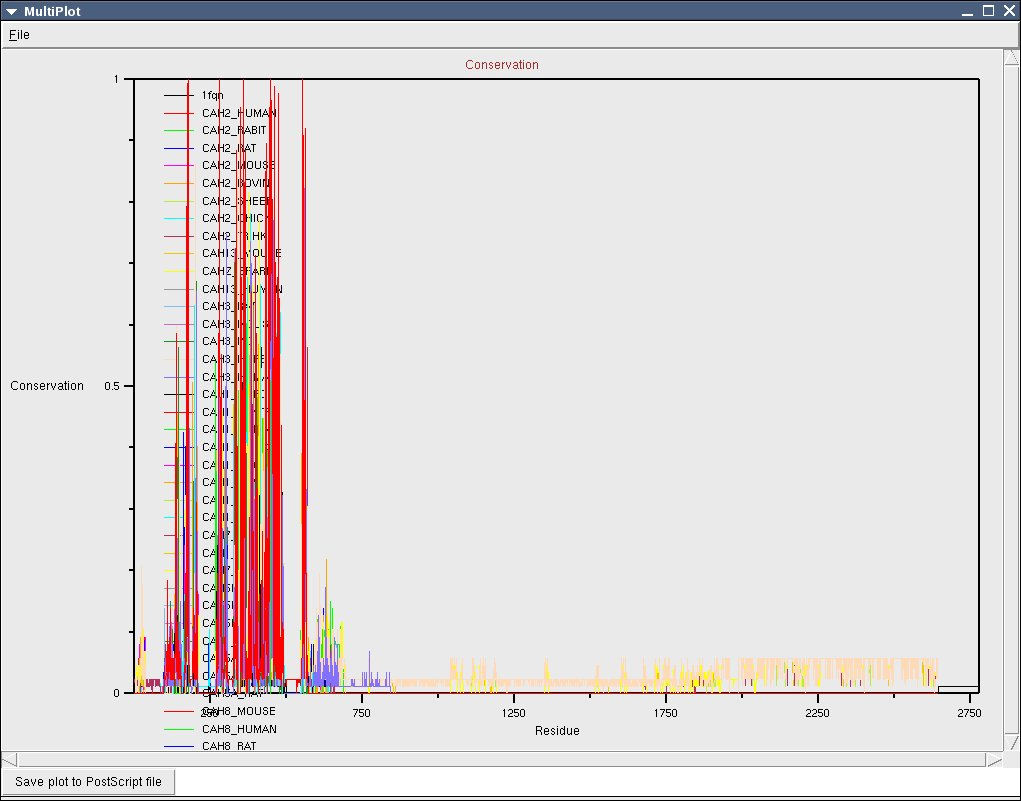
\includegraphics [width=3in]{./pictures/multiPlot.jpg}}
 \caption{Plot Data - Sequence Conservation}
\label{fig:plotData}
\end{figure}
You can \textsf{Plot Data} from the \textsf{Tools} menu in MultiSeq.
Once you choose the sequences or regions you wish to plot, you can
choose the data (such as \textsf{Qres}, \textsf{RMSD}, etc) for each
residue that you want to display.  You can also plot custom data.  The
data graph will then be displayed (see Fig.~\ref{fig:plotData}).  If you
wish, you can create a postscript file for publication.

